\documentclass[conference]{IEEEtran}
\IEEEoverridecommandlockouts
% The preceding line is only needed to identify funding in the first footnote. If that is unneeded, please comment it out.
\usepackage{cite}
\usepackage{amsmath,amssymb,amsfonts}
\usepackage{graphicx}
\usepackage{textcomp}
\usepackage{algorithm}
\usepackage{algpseudocode}
\usepackage[table,xcdraw,dvipsnames]{xcolor}
\usepackage{multirow}
\usepackage[normalem]{ulem}
\useunder{\uline}{\ul}{}

\def\BibTeX{{\rm B\kern-.05em{\sc i\kern-.025em b}\kern-.08em
    T\kern-.1667em\lower.7ex\hbox{E}\kern-.125emX}}

\definecolor{LightGreen}{rgb}{0.9,1,0.9}
\usepackage{hyperref}
\hypersetup{
    colorlinks=true,
    linkcolor=blue,
    filecolor=magenta,      
    urlcolor=blue,
    citecolor = blue,
}

\DeclareMathOperator*{\argmin}{arg\,min}
\DeclareMathOperator*{\argmax}{arg\,max}
    
\begin{document}

\title{Recurrent Inference Machines with Generative Initialization for Image Inverse Problems}
\author{\IEEEauthorblockN{Ernesto Jos\'e Vasquez\textsuperscript{†,$\ast$}, Juan Jos\'e Ribero\textsuperscript{‡,$\ast$}, Emmanuel Martinez\textsuperscript{‡}\&  Henry Arguello
\textsuperscript{‡}}
\IEEEauthorblockA{{\textsuperscript{†}Department of Electrical Engineering}\\
\textsuperscript{‡}Department of Computer Science\\
Universidad Industrial de Santander, Colombia}

\thanks{The authors acknowledge the support of the Office of the Vice President for Research and Extension at Universidad Industrial de Santander (VIE-UIS), which funded this work through project 4765.}
\thanks{\textsuperscript{$\ast$}Both authors contributed equally.}
}

\maketitle

\begin{abstract}
Imaging inverse problems aim to recover a clean image from degraded measurements and are often solved with iterative methods such as Alternating Direction Method of Multipliers (ADMM). Since these problems are ill-posed, ADMM-based reconstruction must be paired with a prior. Generative priors address this by restricting reconstructions to the output of a pretrained generator, which promotes realistic image structure while the solver enforces data consistency. However, many generative prior methods start the latent search from a random code, which is not conditioned on the measurement and can give the solver a poor starting point. Learned initializations improve this starting point, but they are still typically refined with fixed optimization procedures. In this work, we combine a learned generative initialization with Recurrent Inference Machines (RIMs). A fixed encoder-generator pair maps the backprojected measurement to a structured initial estimate, and a RIM refines it using the current reconstruction, a backprojected measurement residual, and a recurrent hidden state. Experiments on single-pixel imaging and super-resolution show that PRIM improves reconstruction quality in the most constrained settings while keeping millisecond-level inference comparable to a standard RIM and substantially faster than ADMM-based baselines.
\end{abstract}

\begin{IEEEkeywords}
Imaging inverse problems, generative priors, recurrent inference machines, algorithm initialization.
\end{IEEEkeywords}

\section{Introduction}
Image inverse problems, such as single-pixel imaging and super-resolution, aim to recover a clean image from a degraded observation \cite{bertero2021introduction}. In practice, this means taking measurements that contain only partial information and trying to rebuild the original image as faithfully as possible. Because the measurements are limited or corrupted, these problems are ill-posed and usually need both a data term and a prior to guide the reconstruction. One of the most common tools for this is the Alternating Direction Method of Multipliers (ADMM)~\cite{neal2011distributed}, since it splits the problem into simpler steps and keeps data consistency under control. This makes it a practical choice when the forward model is known and the reconstruction has to balance fidelity with prior information. In many image restoration settings, this balance is what determines whether the output is only visually plausible or also faithful to the observed measurements.

Recent work has also explored generative priors~\cite{bora2017compressed, latorre2019fast}. In this setting, the solution is restricted to the output of a pretrained generator, which helps preserve realistic image structure and avoid reconstructions that look noisy or unnatural. The idea is to search in the latent space instead of the full image space, which reduces the size of the problem and can improve the final result~\cite{bora2017compressed}. This is especially useful when the measurements are very limited, because the generator acts as a strong prior that narrows the space of possible solutions. Even so, many methods still start from a random latent code, which gives a weak initial point. Other approaches learn that latent initialization from the observation~\cite{gutierrez2025learned}, but they still depend on a fixed solver and hand-designed update rules, so the reconstruction can remain slow and sensitive to the problem setup. In those cases, the quality of the final reconstruction depends not only on the prior, but also on how well the optimization steps are tuned. This means that a good prior alone is not enough if the update process is not able to use it properly.

Recurrent Inference Machines (RIMs) offer a different way to handle the iterative part of the reconstruction~\cite{putzky2017recurrent}. A RIM learns the update process directly from data, using the current estimate, the measurement residual, and a hidden state to produce the next reconstruction. This is useful for inverse problems because the known forward model remains in the loop through the residual, while the update rule is learned from examples instead of being manually fixed. The hidden state also gives the method memory across iterations, allowing later updates to depend on corrections made earlier. In other words, instead of following a fixed rule written by hand, the model learns how to refine the image from examples~\cite{putzky2017recurrent}. This makes the method flexible, but it also means that a poor initial estimate can still slow down or weaken the refinement process, especially when the observation is highly constrained. In practice, this can lead to reconstructions that improve slowly at the beginning or that spend many iterations correcting basic structure before recovering finer details.

\begin{figure*}[!t]
    \centering
    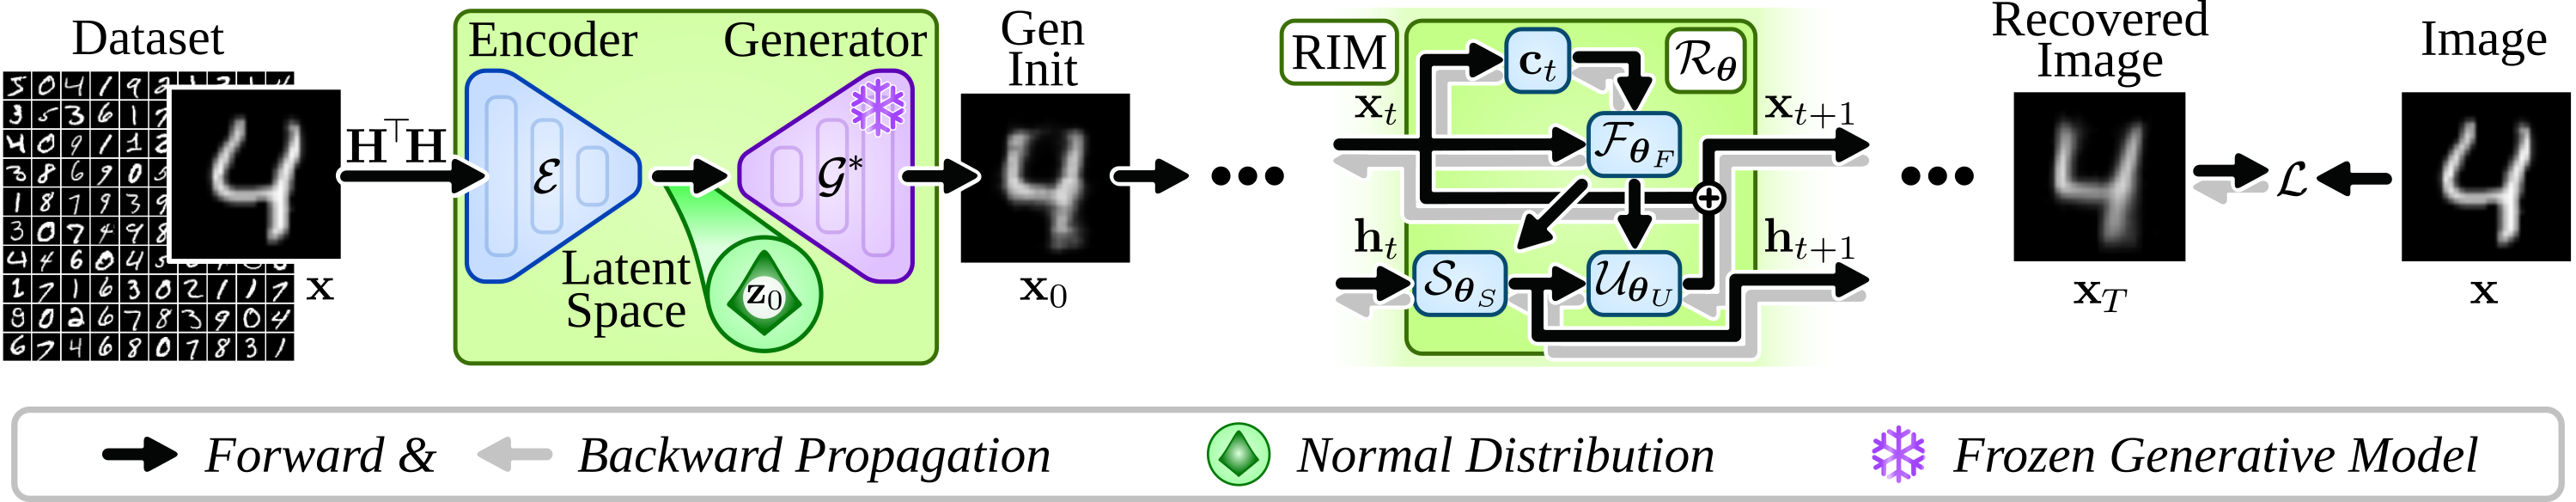
\includegraphics[width=1\textwidth]{figures/fig1.png}
    \caption{\textbf{Overview of the proposed PRIM reconstruction pipeline.} The observation is mapped to $\mathbf{x}_0=\mathcal{G}^{\ast}(\mathcal{E}^{\ast}(\mathbf{H}^{\top}\mathbf{y}))$, and the RIM refines this initialization using the current image, backprojected measurement residual, and hidden state until $\mathbf{x}_T$ is obtained. Finally, the RIM is trained with Eq.~\eqref{eq:rim_training_objective}.}
    \label{fig:method_overview}
    \vspace{-4mm}
\end{figure*}

To address this, we combine a pretrained encoder-generator pair with a RIM. First, the encoder gives an informed latent code and the generator turns it into an initial image estimate. Then the RIM refines that estimate step by step, keeping the structure provided by the generator while learning how to move the reconstruction closer to the observed data. This combination is natural because the generator supplies global image structure, while the RIM can use the forward model residual and its recurrent state to make fast task-aware corrections. This lets the method use the generator as a good starting point and the RIM as a learned refinement stage. As a result, the reconstruction is not rebuilt from scratch, but improved from a point that already carries useful information.

% The main contributions of this work are a RIM-based refinement scheme with generative initialization, a pretrained generator that provides the initial estimate, and an evaluation on single-pixel imaging and super-resolution. Overall, the method gives a more direct inference process than handcrafted ADMM.

% Image inverse problems (single-pixel imaging, super-resolution, etc.) are fundamental in computer vision. The goal is to reconstruct a clean image from an observed degradation. This is referred to as an ill-posed problem.
% Another widely used approach for image reconstruction is based on Generative Models (GAN, VAE, diffusion models, etc.). With this approach, the goal is to optimize a latent representation (z), in which the generated image G(z) is consistent with the observations.

% These generative models are often used with solvers (ADMM, etc.) to enforce consistency with the data during reconstruction. In particular, ADMM is one of the most widely used optimization frameworks for inverse problems, as it allows separating data fidelity and prior terms in a flexible manner. While the generated image is highly realistic, it is often biased toward the training distribution and may not be fully consistent with the observed measurements.

% In generative-based approaches, the latent space is often initialized either randomly, leading to poor starting points, or through learned strategies that require careful parameter tuning and may result in increased computational cost.
% One limitation of these solvers is that they are again manually designed algorithms, relying on fixed update rules and manually tuned parameters, which may limit their adaptability and performance.

% A more recent approach is Recurrent Inference Machines (RIMs), which learn the iterative reconstruction process using likelihood gradients, but also presents some problems, such as the model’s output diverging from the actual data, since it depends on the initial estimate.

% To address these limitations, we propose a new perspective: instead of using RIMs as standalone image reconstruction models, we use them to refine the output of a generative model. In contrast to ADMM-based optimization, we replace the hand-crafted solver with a learned RIM-based inference process.
% In this way, the generative model provides a realistic initial estimate for the RIM, mitigating divergence, while the RIM iteratively improves data fidelity, reducing the reliance on hand-crafted solvers.

% Contributions:

% •	A simple and effective extension of RIM 
% •	Application to single-pixel imaging and super-resolution tasks 
% •	A better initialization strategy based on a pretrained generator and encoder

\section{Inverse Problems with Generative Priors}

\subsection{Problem Formulation}

Let $\mathbf{x} \in \mathbb{R}^{n}$ denote a vectorized image and $\mathbf{y} \in \mathbb{R}^{m}$ its corresponding observation, with $m \leq n$. The acquisition process is modeled as
\vspace{-2mm}
\begin{equation}
    \mathbf{y} = \mathbf{H}\mathbf{x} + \boldsymbol{\eta},
    \label{eq:forward_model}
\end{equation}
where $\mathbf{H} \in \mathbb{R}^{m \times n}$ is the forward operator and 
$\boldsymbol{\eta} \sim \mathcal{N}(\mathbf{0},\sigma^2\mathbf{I})$ is additive Gaussian noise. Recovering $\mathbf{x}$ from $\mathbf{y}$ is generally ill-posed and can be formulated as
\vspace{-2mm}
\begin{equation}
    \mathbf{x}^{\ast} \in 
    \argmin_{\mathbf{x}}
    f(\mathbf{x}) + \lambda g(\mathbf{x}),
    \label{eq:inverse_problem}
    \vspace{-2mm}
\end{equation}
where $f(\mathbf{x})=\|\mathbf{y}-\mathbf{H}\mathbf{x}\|_2^2$ enforces data fidelity, 
$g(\mathbf{x})$ encodes prior information, and $\lambda>0$ balances both terms.

\subsection{Generative Priors}

Deep generative models can act as priors by restricting the solution to the range of a pretrained generator $\mathcal{G}^{\ast}:\mathbb{R}^{d}\rightarrow\mathbb{R}^{n}$, where 
$\mathbf{z}\in\mathbb{R}^{d}$ is a low-dimensional latent vector~\cite{bora2017compressed}. Thus, the recovered image is represented as $\mathbf{x}=\mathcal{G}^{\ast}(\mathbf{z})$, and the inverse problem can be written as
\vspace{-2mm}
\begin{equation}
    \mathbf{z}^{\ast} \in 
    \argmin_{\mathbf{z}}
    \|\mathbf{y}-\mathbf{H}\mathcal{G}^{\ast}(\mathbf{z})\|_2^2 + \lambda g(\mathbf{z}).
    \label{eq:generative_prior}
    \vspace{-2mm}
\end{equation}
This reduces the search space and promotes reconstructions aligned with the learned image manifold. Here, $g(\mathbf{z})$ is a regularizer in the latent space, so the optimization favors latent codes that remain compatible with the pretrained generator.

ADMM-based approaches further introduce both image and latent variables~\cite{gutierrez2025learned},
\vspace{-2mm}
\begin{equation}
    \{\mathbf{x}^{\ast},\mathbf{z}^{\ast}\}
    \in
    \argmin_{\mathbf{x},\mathbf{z}}
    f(\mathbf{x}) + g(\mathbf{z})
    \quad
    \text{s.t.}
    \quad
    \mathbf{x}=\mathcal{G}^{\ast}(\mathbf{z}),
    \label{eq:admm_gp}
    \vspace{-2mm}
\end{equation}
allowing data consistency to be handled in the image domain while the generator constrains the solution through the latent space~\cite{gutierrez2025learned}. In this formulation, $\mathbf{x}$ is the image variable and $\mathbf{z}$ is the latent variable linked by the constraint $\mathbf{x}=\mathcal{G}^{\ast}(\mathbf{z})$.

Recently, Guti\'errez Rengifo et al.~\cite{gutierrez2025learned} improved this framework by replacing random latent initialization with a learned data-dependent initialization, $\mathbf{z}_0 = \mathcal{E}^{\ast}(\mathbf{H}^{\top}\mathbf{y})$, $\mathbf{x}_0 = \mathcal{G}^{\ast}(\mathbf{z}_0)$. Here, $\mathcal{E}^{\ast}$ maps a backprojected observation into the latent space of the fixed generator $\mathcal{G}^{\ast}$. However, the reconstruction is still performed using a hand-designed ADMM solver, which depends on manually defined update rules, hyperparameters, and a fixed number of iterations. This motivates replacing the optimization solver with a learned iterative framework, such as RIMs, which learn the inference dynamics from data while preserving the structure of the inverse problem \cite{putzky2017recurrent}. For the proposed setting, this is attractive because the same recurrent cell can repeatedly use the measurement residual while learning how much of each correction should be applied at each step.

\section{Recurrent Inference Machine-based Generative Refinement}

The proposed method, summarized in Fig.~\ref{fig:method_overview}, builds on learned generative initialization frameworks by replacing the hand-designed ADMM solver with a learned iterative refinement model based on RIMs. Given an observation $\mathbf{y}$, we first backproject the measurement and obtain a structured initialization from a pretrained encoder-generator pair, $\mathbf{z}_0 = \mathcal{E}^{\ast}(\mathbf{H}^{\top}\mathbf{y})$, $\mathbf{x}_0 = \mathcal{G}^{\ast}(\mathbf{z}_0)$, where $\mathcal{G}^{\ast}$ is the fixed generator and $\mathcal{E}^{\ast}$ maps the backprojected observation into the generator latent space. Instead of using $\mathbf{x}_0$ to initialize an ADMM solver, we use it as the starting point of a RIM-based reconstruction process. This shifts the task from reconstructing the image from scratch to refining a structured estimate using backprojected measurement residuals and recurrent memory.

Starting from $\mathbf{x}_0$, the RIM iteratively updates the reconstruction by combining the current estimate with information from the forward model. For the data fidelity term $f(\mathbf{x})=\|\mathbf{y}-\mathbf{H}\mathbf{x}\|_2^2$, we define the backprojected measurement residual at iteration $t$ as
\vspace{-2mm}
\begin{equation}
    \mathbf{c}_t = \mathbf{H}^{\top}(\mathbf{y}-\mathbf{H}\mathbf{x}_t),
    \label{eq:correction}
    \vspace{-2mm}
\end{equation}
which is proportional to the negative gradient of $f(\mathbf{x})$, since $\nabla f(\mathbf{x}_t)=2\mathbf{H}^{\top}(\mathbf{H}\mathbf{x}_t-\mathbf{y})$. The recurrent refinement is modeled as
\vspace{-2mm}
\begin{equation}
    \mathbf{x}_{t+1}, \mathbf{h}_{t+1} 
    =
    \mathcal{R}_{\boldsymbol{\theta}}
    \left(
        \mathbf{x}_{t}, 
        \mathbf{c}_{t}, 
        \mathbf{h}_{t}
    \right),
    \label{eq:rim_update}
    \vspace{-2mm}
\end{equation}
where $\mathbf{h}_t$ is the hidden state and $\mathcal{R}_{\boldsymbol{\theta}}$ denotes the complete RIM cell.
In our implementation, $\mathcal{R}_{\boldsymbol{\theta}}$ is parameterized by three learnable components, a convolutional feature extractor $\mathcal{F}_{\boldsymbol{\theta}_F}$, a recurrent state update module  $\mathcal{S}_{\boldsymbol{\theta}_S}$, and an image update head $\mathcal{U}_{\boldsymbol{\theta}_U}$. Specifically,
\vspace{-2mm}
\begin{align}
    \mathbf{q}_t 
    &= 
    \mathcal{F}_{\boldsymbol{\theta}_F}
    \left(
        [\mathbf{x}_t,\mathbf{c}_t]
    \right), \\
    \mathbf{h}_{t+1} 
    &= 
    \mathcal{S}_{\boldsymbol{\theta}_S}
    \left(
        \mathbf{q}_t,\mathbf{h}_t
    \right), \\
    \Delta \mathbf{x}_t 
    &= 
    \mathcal{U}_{\boldsymbol{\theta}_U}
    \left(
        [\mathbf{q}_t,\mathbf{h}_{t+1}]
    \right), \\
    \mathbf{x}_{t+1} 
    &= 
    \mathbf{x}_t + \alpha \Delta \mathbf{x}_t.
    \vspace{-2mm}
\end{align}
Therefore, the full recurrent operator can be written compactly as
\vspace{-2mm}
\begin{equation}
    \mathcal{R}_{\boldsymbol{\theta}}
    =
    \left\{
    \mathcal{F}_{\boldsymbol{\theta}_F},
    \mathcal{S}_{\boldsymbol{\theta}_S},
    \mathcal{U}_{\boldsymbol{\theta}_U},
    \alpha
    \right\},
    \qquad
    \boldsymbol{\theta} =
    \{\boldsymbol{\theta}_F,\boldsymbol{\theta}_S,\boldsymbol{\theta}_U\},
    \vspace{-2mm}
\end{equation}
where $[\cdot,\cdot]$ denotes channel-wise concatenation and $\alpha=0.1$ is fixed in our implementation.

The RIM parameters are learned by minimizing the reconstruction error over the unrolled refinement trajectory
\begin{equation}
    \boldsymbol{\theta}^{\ast}
    \in
    \argmin_{\boldsymbol{\theta}}
    \mathbb{E}_{(\mathbf{x},\mathbf{y})\sim \mathcal{D}}
    \left[
    \sum_{t=1}^{T}
    w_t
    \left\|
        \mathbf{x}_t - \mathbf{x}
    \right\|_2^2
    \right],
    \label{eq:rim_training_objective}
\end{equation}
where the sequence $\{\mathbf{x}_t\}_{t=0}^{T}$ is generated from 
$\mathbf{x}_0=\mathcal{G}^{\ast}(\mathcal{E}^{\ast}(\mathbf{H}^{\top}\mathbf{y}))$ using the recurrent update in Eq.~\eqref{eq:rim_update}. Here, $w_t \geq 0$, $\sum_{t=1}^{T}w_t=1$, and $\mathcal{D}$ denotes the training distribution. The rollout is performed by unrolling the RIM for $T$ steps from the initialization $\mathbf{x}_0$. The training flow is summarized in Algorithm~\ref{alg:training_framework}. The only change with respect to a base RIM is the initialization of $\mathbf{x}_0$; the hidden state is initialized as $\mathbf{h}_0=\mathbf{0}$.

\begin{algorithm}[t]
\caption{Training procedure for PRIM}
\label{alg:training_framework}
\small
\begin{algorithmic}[1]
\Require Training pair $(\mathbf{x}^{\ast},\mathbf{y})$, encoder $\mathcal{E}^{\ast}$, generator $\mathcal{G}^{\ast}$, RIM parameters $\boldsymbol{\theta}$, number of steps $T$
\State $\mathbf{z}_0 \gets \mathcal{E}^{\ast}(\mathbf{H}^{\top}\mathbf{y})$
\State $\mathbf{x}_0 \gets \mathcal{G}^{\ast}(\mathbf{z}_0)$
\State $\mathbf{h}_0 \gets \mathbf{0}$
\For{$t = 0,\ldots,T-1$}
    \State $\mathbf{c}_t \gets \mathbf{H}^{\top}(\mathbf{y}-\mathbf{H}\mathbf{x}_t)$
    \State $(\mathbf{x}_{t+1},\mathbf{h}_{t+1}) \gets \mathcal{R}_{\boldsymbol{\theta}}(\mathbf{x}_t,\mathbf{c}_t,\mathbf{h}_t)$
\EndFor
\State Update $\boldsymbol{\theta}$ using $\sum_{t=1}^{T} w_t \|\mathbf{x}_t-\mathbf{x}^{\ast}\|_2^2$
\State \Return $\mathbf{x}_T$
\end{algorithmic}
\end{algorithm}

The proposed formulation preserves the structured prior provided by the generator while replacing the fixed ADMM updates with a learned solver. As a result, the refinement process can be optimized directly from data, improving reconstruction quality and reducing the number of iterations required at inference time.

% \section{Proposed Method}

% Our method consists of two stages. First, a generative initialization stage, whose objective is to optimize the encoder that maps the data $y$ into a latent space $z$ compatible with a pre-trained generator, producing an initial estimate of the image. Second, a RIM-based refinement stage, where, rather than being a reconstruction task starting from scratch, RIM functions as a refinement model by leveraging the initialization from stage 1.


% \subsection{Stage 1: Learned Generative Initialization}

% The goal of the first stage is to improve the initial estimate $x_0$ used by the RIM method.

% We start from the corresponding observation $y$. To obtain a better initialization, we use a pretrained generator $G_\star$ together with an encoder $E_\star$. The encoder maps the observation to the latent space:
% \begin{equation}
% z = E_\star(y),
% \end{equation}
% and the initial image is obtained as
% \begin{equation}
% x_0 = G_\star(z).
% \end{equation}

% The encoder is trained while keeping the generator fixed, so that $G_\star(E_\star(o))$ approximates the ground-truth image. In this way, we obtain an initialization that is more informative than the direct backprojection and that lies on the manifold induced by the generator.

% This stage allows us to shift the problem from a difficult reconstruction task to a refinement problem around a structured initial solution.

% \subsection{Stage 2: RIM Refinement}

% Starting from $x_0$, we apply a Recurrent Inference Machine (RIM) to iteratively refine the reconstruction.
% \begin{equation}
% x_0 = G_\star(E_\star(y))
% \end{equation}
% Unlike standard RIM, which typically starts from a poor initialization (e.g., $o$), our method starts from an estimate that already captures the global structure of the image.
% \subsubsection{Data-Consistency Correction} 
% At iteration t, the correction term is
% \begin{equation}
% c_t = H^T(y - Hx_t),
% \end{equation}

% \subsubsection{Recurrent Update}

% The current implementation uses a convolutional encoder, a convolutional GRU state, and an update head. If $s_t$ denotes the hidden state, then the recurrent dynamics are:

% \begin{equation}
% f_t = F_\boldsymbol{\theta}([x_t,c_t]),
% \end{equation}
% \begin{equation}
% s_{t+1} = S_\boldsymbol{\theta}(f_t,s_t),
% \end{equation}
% \begin{equation}
% \Delta x_t = \alpha U_\boldsymbol{\theta}([f_t,s_{t+1}]),
% \end{equation}

% where [.,.] denotes channel concatenation and $\alpha > 0 $ is the learned step scale. 

% ... Duda intervalo

% The image update is:

% \begin{equation}
% x_{t+1} = x_t + R_\boldsymbol{\theta}(x_t, H^\top (y - Hx_t)),
% \end{equation}

% \subsubsection{Training Loss}
% The RIM is trained with a multi-step reconstruction loss. If $x^\star$ is the ground-truth image and ${w_t}_{t=1}^{T}$ are nonnegative weights satisfying $\sum $ 




% At each iteration, the RIM uses data-consistency information to correct the current estimate. This allows the model to focus on recovering fine details and improving consistency with the measurements.

% In this sense, the proposed method can be seen as a modified RIM, where the task shifts from reconstructing the image from scratch to refining a structured initial estimate.



% \subsection{Summary}

% The proposed approach combines:
% \begin{itemize}
%     \item a \textbf{generative prior}, enforced through the pretrained generator $G_\star$, and
%     \item a \textbf{data-consistency refinement}, enforced through the RIM updates.
% \end{itemize}

% This two-stage design separates prior modeling from iterative correction, leading to improved reconstruction quality and faster convergence.

% \subsection{Single-Pixel Imaging Case}

% In the single-pixel imaging (SPI) setting, the observation is obtained through a linear sensing process:
% \[
% y = Hx + \eta,
% \]
% where $H$ is a (typically underdetermined) sensing matrix and $m \ll n$. In our setup, $H$ corresponds to a row-truncated Hadamard matrix, which compresses the image into a reduced set of measurements.

% The gradient of the data-fidelity term is given by
% \[
% H^\top (Hx_t - y),
% \]
% which measures the inconsistency between the current estimate and the measurements.

% This leads to a correction step that pushes the reconstruction toward agreement with the sensing model. Unlike the denoising case, the update is not a simple pixel-wise operation, since it involves both projection and backprojection through $H$ and $H^\top$.

% As a result, the reconstruction process must iteratively balance measurement consistency and image structure, making SPI a more challenging inverse problem.


% \subsection{Super-Resolution Case} \label{SCM}

% In super-resolution, the gradient involves both the degradation operator and an upsampling process.

% Unlike denoising, there is no simple closed-form correction.

% Instead, the correction step is formulated as an optimization problem.

% We solve this problem using a few steps of gradient descent.


% \subsection{Algorithm}

% For SPI:
% \begin{equation}
% o = \frac{1}{n} H^\top y,
% \end{equation}
% which corresponds to a normalized backprojection. This already contains some information about the original image, but it is still a poor estimate due to the ill-posed nature of the inverse problem.


% \subsection{Figures and Tables}

\begin{figure}[!b]
    \vspace{-4mm}
    \centering
    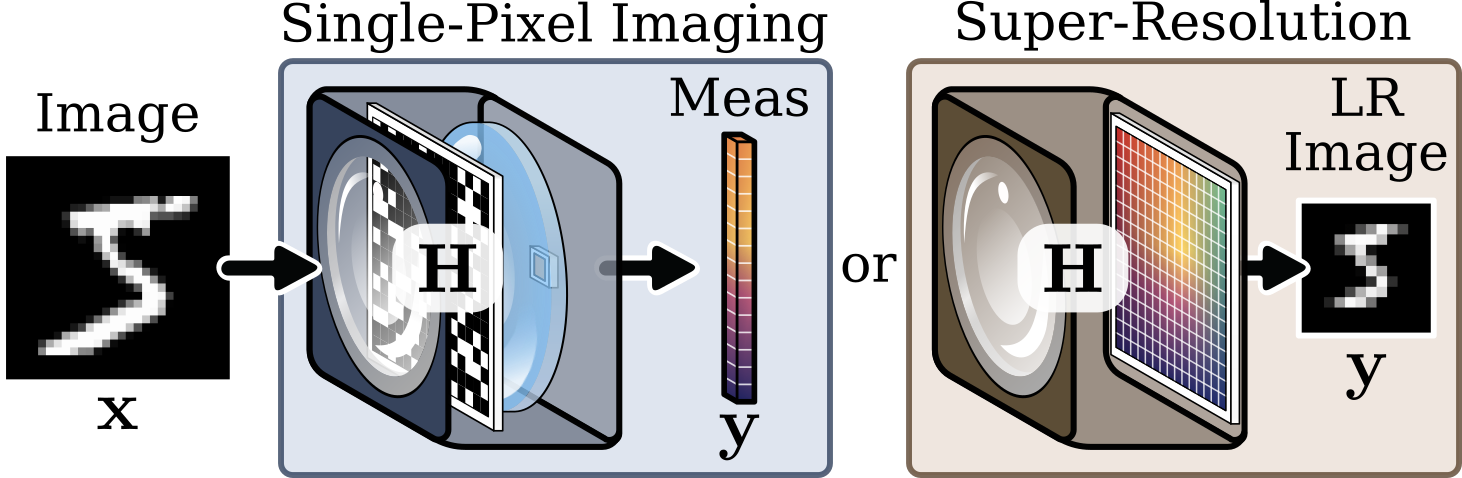
\includegraphics[width=0.46\textwidth]{figures/fig2.png}
    \caption{\textbf{Inverse-problem settings used in the experiments.} In SPI, the sensing matrix $\mathbf{H}$ maps the image to compressive measurements $\mathbf{y}$. In SR, $\mathbf{H}$ is a downsampling operator that produces a low-resolution observation from the target image.}
    \label{fig:inverse_problem_settings}
    \vspace{-4mm}
\end{figure}

\begin{table}[b!]
\caption{Quantitative reconstruction performance on the MNIST test set. Higher PSNR and SSIM values indicate better reconstruction quality, whereas lower MSE and MAE values indicate lower reconstruction error. Best results are shown in bold with green shading, and second best results are underlined with blue shading.}
\label{tab:reconstruction_metrics}
\setlength{\tabcolsep}{12pt}
\renewcommand{\arraystretch}{1.3}
\begin{tabular}{|ccccc|}
\hline \hline
\multicolumn{5}{|c|}{\textbf{Single-Pixel Imaging}}                                                                                                                                                                                                                         \\ \hline
\multicolumn{1}{|c|}{\textbf{Method}}                         & \multicolumn{1}{c|}{\textbf{PSNR}}                          & \multicolumn{1}{c|}{\textbf{SSIM}}                           & \multicolumn{1}{c|}{\textbf{MSE}}                            & \textbf{MAE}    \\ \hline
\multicolumn{5}{|c|}{\textbf{$\kappa = 0.01$}}                                                                                                                                                                                                                              \\ \hline
\multicolumn{1}{|c|}{\textbf{EADMM}}                          & \multicolumn{1}{c|}{12.58}                                  & \multicolumn{1}{c|}{0.4591}                                  & \multicolumn{1}{c|}{0.0652}                                  & 0.1078          \\ \hline
\multicolumn{1}{|c|}{\textbf{GANI}}                           & \multicolumn{1}{c|}{17.81}                                  & \multicolumn{1}{c|}{0.7410}                                  & \multicolumn{1}{c|}{0.0217}                                  & 0.0585          \\ \hline
\multicolumn{1}{|c|}{\textbf{PEADMM}} & \multicolumn{1}{c|}{17.99}          & \multicolumn{1}{c|}{\cellcolor[HTML]{DDEBF7}{\ul 0.7466}}          & \multicolumn{1}{c|}{0.0209}          & \cellcolor[HTML]{DDEBF7}{\ul 0.0577}    \\ \hline
\multicolumn{1}{|c|}{\textbf{RIM}}    & \multicolumn{1}{c|}{\cellcolor[HTML]{DDEBF7}{\ul 18.29}}    & \multicolumn{1}{c|}{0.7375}    & \multicolumn{1}{c|}{\cellcolor[HTML]{DDEBF7}{\ul 0.0197}}    & 0.0589          \\ \hline
\multicolumn{1}{|c|}{\textbf{PRIM}}   & \multicolumn{1}{c|}{\cellcolor[HTML]{E2EFDA}\textbf{18.96}} & \multicolumn{1}{c|}{\cellcolor[HTML]{E2EFDA}\textbf{0.7651}} & \multicolumn{1}{c|}{\cellcolor[HTML]{E2EFDA}\textbf{0.0182}} & \cellcolor[HTML]{E2EFDA}\textbf{0.0545} \\ \hline
\multicolumn{5}{|c|}{\textbf{$\kappa = 0.05$}}                                                                                                                                                                                                                              \\ \hline
\multicolumn{1}{|c|}{\textbf{EADMM}}                          & \multicolumn{1}{c|}{21.30}                                  & \multicolumn{1}{c|}{0.8607}                                  & \multicolumn{1}{c|}{0.0113}                                  & 0.0359          \\ \hline
\multicolumn{1}{|c|}{\textbf{GANI}}                           & \multicolumn{1}{c|}{22.54}                                  & \multicolumn{1}{c|}{0.9037}                                  & \multicolumn{1}{c|}{0.0068}                                  & 0.0295          \\ \hline
\multicolumn{1}{|c|}{\textbf{PEADMM}} & \multicolumn{1}{c|}{25.23}          & \multicolumn{1}{c|}{0.9438}    & \multicolumn{1}{c|}{0.0037}          & 0.0221          \\ \hline
\multicolumn{1}{|c|}{\textbf{RIM}}    & \multicolumn{1}{c|}{\cellcolor[HTML]{DDEBF7}{\ul 30.29}}    & \multicolumn{1}{c|}{\cellcolor[HTML]{DDEBF7}{\ul 0.9802}}          & \multicolumn{1}{c|}{\cellcolor[HTML]{DDEBF7}{\ul 0.0012}}    & \cellcolor[HTML]{DDEBF7}{\ul 0.0119}    \\ \hline
\multicolumn{1}{|c|}{\textbf{PRIM}}   & \multicolumn{1}{c|}{\cellcolor[HTML]{E2EFDA}\textbf{30.80}} & \multicolumn{1}{c|}{\cellcolor[HTML]{E2EFDA}\textbf{0.9839}} & \multicolumn{1}{c|}{\cellcolor[HTML]{E2EFDA}\textbf{0.0011}} & \cellcolor[HTML]{E2EFDA}\textbf{0.0110} \\ \hline
\multicolumn{5}{|c|}{\textbf{Super-Resolution}}                                                                                                                                                                                                                             \\ \hline
\multicolumn{1}{|c|}{\textbf{Method}}                         & \multicolumn{1}{c|}{\textbf{PSNR}}                          & \multicolumn{1}{c|}{\textbf{SSIM}}                           & \multicolumn{1}{c|}{\textbf{MSE}}                            & \textbf{MAE}    \\ \hline
\multicolumn{5}{|c|}{\textbf{$s = \times 8$}}                                                                                                                                                                                                                               \\ \hline
\multicolumn{1}{|c|}{\textbf{EADMM}}                          & \multicolumn{1}{c|}{11.58}                                  & \multicolumn{1}{c|}{0.3809}                                  & \multicolumn{1}{c|}{0.0779}                                  & 0.1227          \\ \hline
\multicolumn{1}{|c|}{\textbf{GANI}}                           & \multicolumn{1}{c|}{19.69}                                  & \multicolumn{1}{c|}{0.8316}                                  & \multicolumn{1}{c|}{0.0141}                                  & 0.0440          \\ \hline
\multicolumn{1}{|c|}{\textbf{PEADMM}} & \multicolumn{1}{c|}{19.95}          & \multicolumn{1}{c|}{0.8383}          & \multicolumn{1}{c|}{0.0134}          & 0.0429          \\ \hline
\multicolumn{1}{|c|}{\textbf{RIM}}    & \multicolumn{1}{c|}{\cellcolor[HTML]{DDEBF7}{\ul 20.49}}          & \multicolumn{1}{c|}{\cellcolor[HTML]{DDEBF7}{\ul 0.8497}}          & \multicolumn{1}{c|}{\cellcolor[HTML]{DDEBF7}{\ul 0.0122}}          & \cellcolor[HTML]{DDEBF7}{\ul 0.0417}          \\ \hline
\multicolumn{1}{|c|}{\textbf{PRIM}}   & \multicolumn{1}{c|}{\cellcolor[HTML]{E2EFDA}\textbf{20.91}} & \multicolumn{1}{c|}{\cellcolor[HTML]{E2EFDA}\textbf{0.8590}} & \multicolumn{1}{c|}{\cellcolor[HTML]{E2EFDA}\textbf{0.0117}} & \cellcolor[HTML]{E2EFDA}\textbf{0.0389} \\ \hline
\multicolumn{5}{|c|}{\textbf{$s = \times 4$}}                                                                                                                                                                                                                               \\ \hline
\multicolumn{1}{|c|}{\textbf{EADMM}}                          & \multicolumn{1}{c|}{16.99}                                  & \multicolumn{1}{c|}{0.6837}                                  & \multicolumn{1}{c|}{0.0319}                                  & 0.0646          \\ \hline
\multicolumn{1}{|c|}{\textbf{GANI}}                           & \multicolumn{1}{c|}{24.67}                                  & \multicolumn{1}{c|}{0.9395}                                  & \multicolumn{1}{c|}{0.0043}                                  & 0.0233          \\ \hline
\multicolumn{1}{|c|}{\textbf{PEADMM}} & \multicolumn{1}{c|}{25.75}          & \multicolumn{1}{c|}{0.9525}          & \multicolumn{1}{c|}{0.0033}          & 0.0206          \\ \hline
\multicolumn{1}{|c|}{\textbf{RIM}}    & \multicolumn{1}{c|}{\cellcolor[HTML]{DDEBF7}{\ul 29.24}}    & \multicolumn{1}{c|}{\cellcolor[HTML]{E2EFDA}\textbf{0.9797}} & \multicolumn{1}{c|}{\cellcolor[HTML]{E2EFDA}\textbf{0.0016}} & \cellcolor[HTML]{DDEBF7}{\ul 0.0128}    \\ \hline
\multicolumn{1}{|c|}{\textbf{PRIM}}   & \multicolumn{1}{c|}{\cellcolor[HTML]{E2EFDA}\textbf{29.26}} & \multicolumn{1}{c|}{\cellcolor[HTML]{DDEBF7}{\ul 0.9790}}    & \multicolumn{1}{c|}{\cellcolor[HTML]{DDEBF7}{\ul 0.0017}}    & \cellcolor[HTML]{E2EFDA}\textbf{0.0127} \\ \hline \hline
\end{tabular}
\end{table}

\section{Experiments \& Results}

\begin{figure*}[!t]
    \centering
    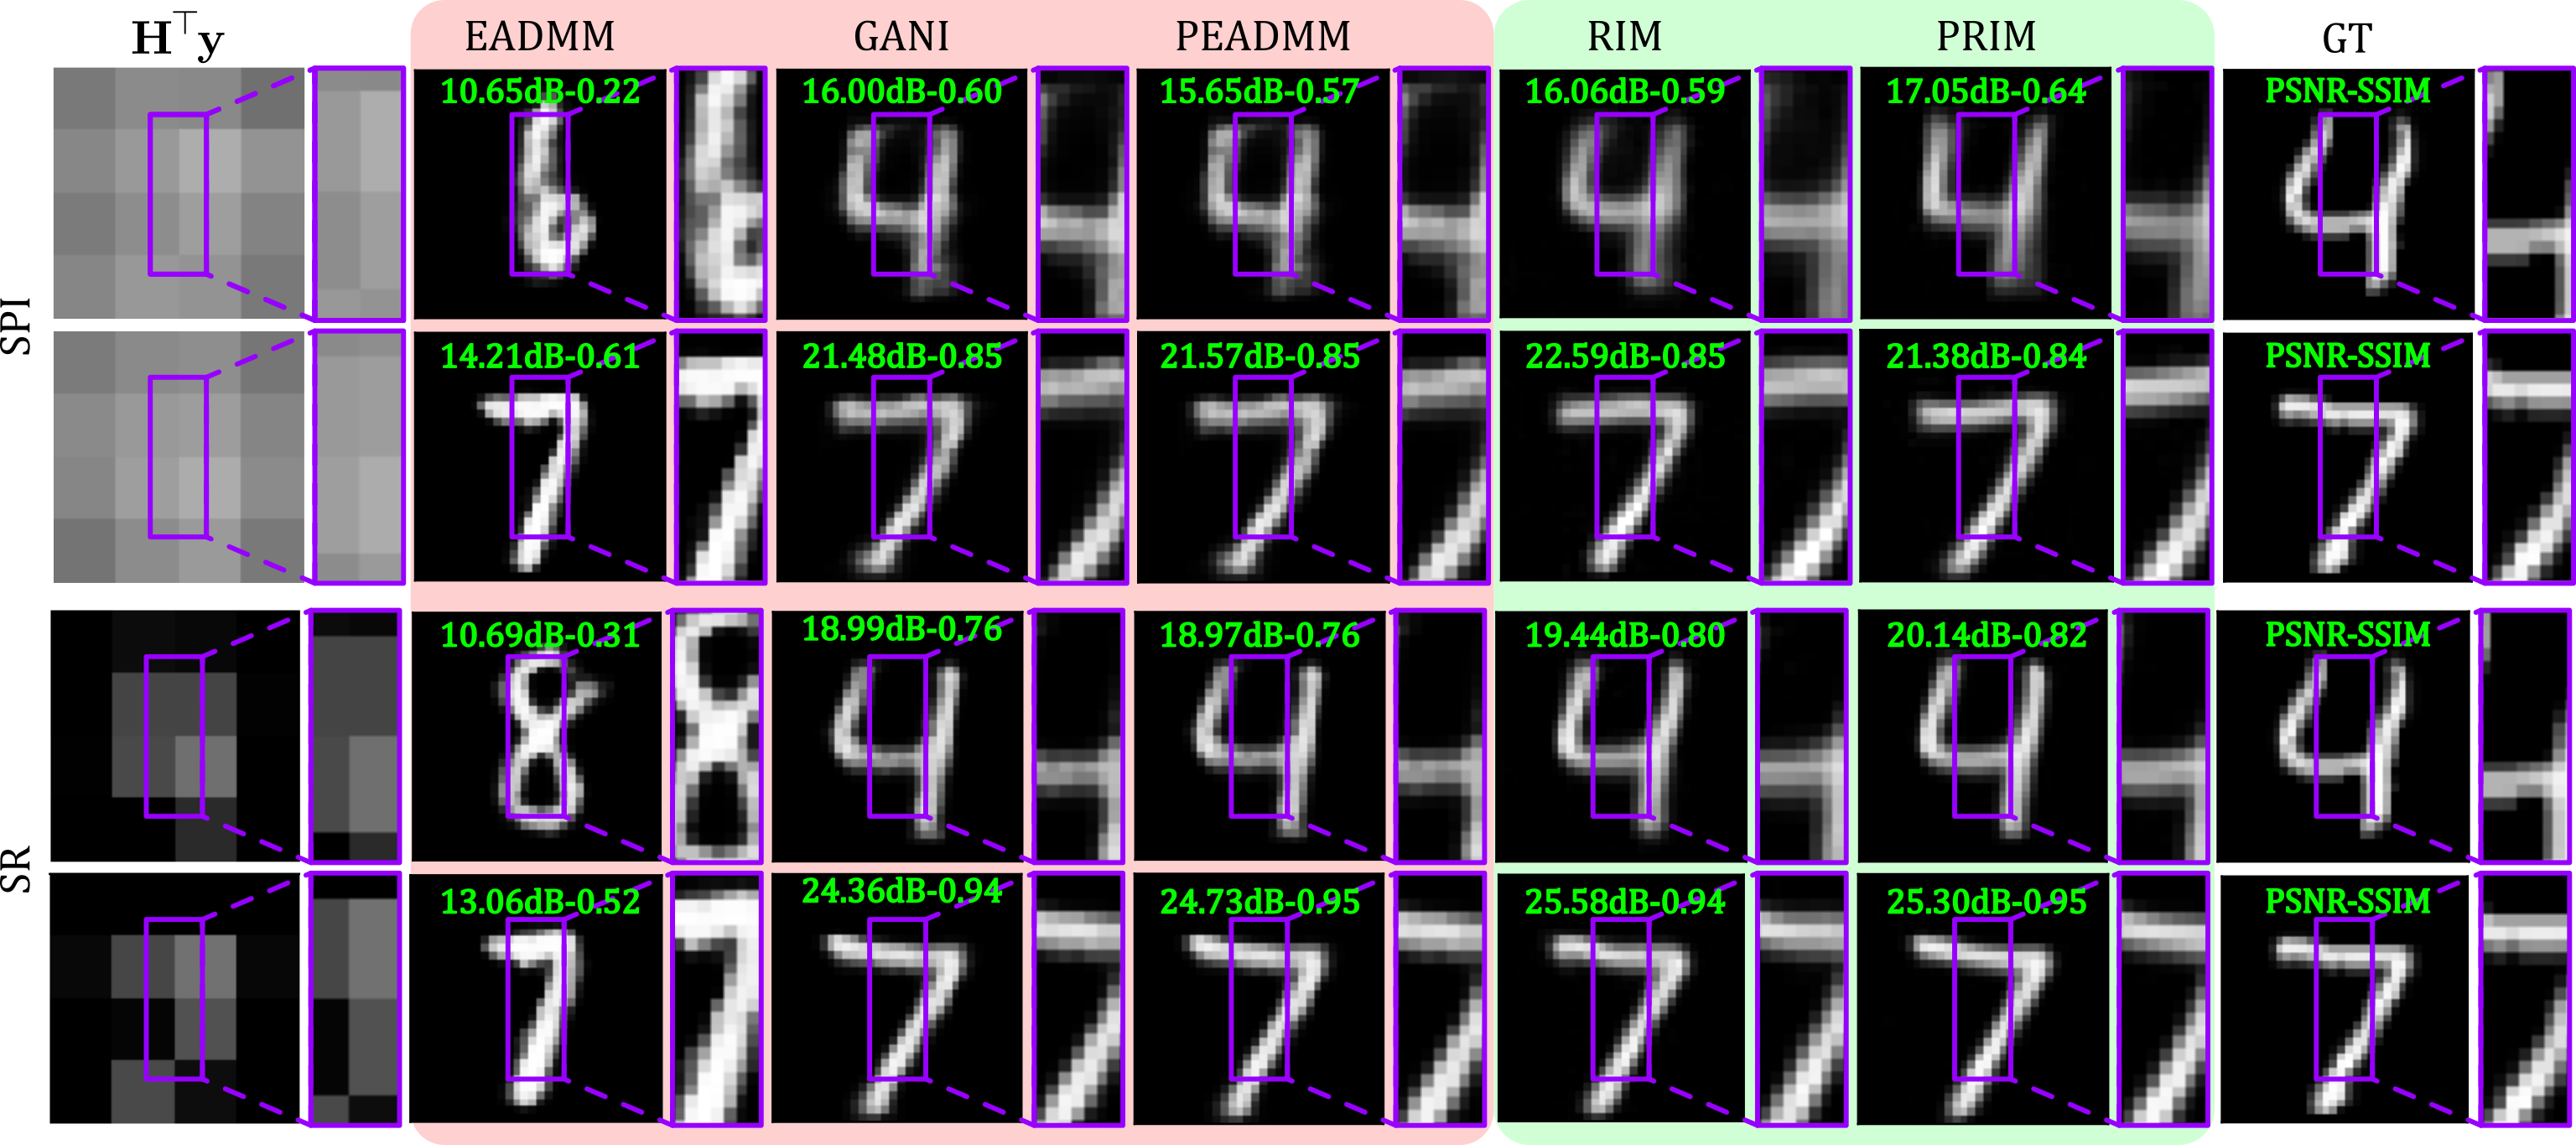
\includegraphics[width=1\textwidth]{figures/fig3.png}
    \caption{\textbf{Qualitative reconstruction comparison on MNIST test samples.} Representative SPI examples with compression ratio $\kappa=0.01$ and SR examples with scale factor $\times 8$ are shown with their corresponding backprojections or low-resolution observations, method reconstructions, and ground truth images.}
    \label{fig:qualitative_results}
    \vspace{-4mm}
\end{figure*}

We evaluate the proposed method on MNIST digit images resized from $28\times28$ to $32\times32$ pixels. From the original 60,000 training images, 5,000 samples are used for validation, and the remaining samples are used for training. All reported quantitative results are computed on the full 10,000 image test set. The two inverse-problem settings are illustrated in Fig.~\ref{fig:inverse_problem_settings}. In SPI, $\mathbf{H}$ is a row-truncated Hadamard matrix with zig-zag ordered rows and $\kappa=m/n\in\{0.01,0.05\}$ \cite{zhang2017hadamard}. The image-domain observation is $\mathbf{H}^{\top}\mathbf{y}/n$. In SR, the forward operator applies an average filter of size $s\times s$ and stride $s$, with $s\in\{\times8,\times4\}$ \cite{conde2025ntire}. We compare PRIM against EADMM, PEADMM, GANI, and a standard RIM initialized from the backprojection. Reconstruction quality is measured with PSNR, SSIM, MSE, and MAE \cite{wang2004image}, and runtime is measured per image on an NVIDIA RTX 3090 GPU \cite{imambi2021pytorch}.

\subsection{Generative initialization}

The generative initialization follows~\cite{gutierrez2025learned}. A WGAN-GP generator is trained on $32\times32$ MNIST digits, and task-specific encoders map the backprojection to the generator latent space. The fixed encoder-generator pair defines GANI and initializes PRIM as $\mathbf{x}_0=\mathcal{G}^{\ast}(\mathcal{E}^{\ast}(\mathbf{H}^{\top}\mathbf{y}))$. PEADMM uses the same encoder output only as an ADMM latent initialization. Both RIM and PRIM use the same image-space RIM. It contains a two-layer convolutional input encoder, a ConvGRU with 32 hidden channels, and a two-layer update head, and is unrolled for $T=10$ steps. The model is trained with Adam using learning rate $10^{-3}$, batch size 128, and gradient clipping at norm 1.0.

% \textcolor{red}{The pretrained generator $\mathcal{G}^{\ast}$ and encoders $\mathcal{E}^{\ast}$ are used as fixed components inherited from the learned latent-space initialization framework \cite{}. They provide the feed-forward GANI baseline, the learned initialization used by PEADMM, and the generative initialization used by PRIM. Since these components are not the main contribution of this work, they are kept fixed across methods, and the comparison focuses on the reconstruction stage: handcrafted ADMM refinement versus learned RIM-based refinement.}

\subsection{Main results}

Quantitative reconstruction results are summarized in Tab.~\ref{tab:reconstruction_metrics}. In the most compressed SPI setting ($\kappa=0.01$), PRIM obtains the best score in all reported metrics, improving the standard RIM from 18.29 dB to 18.96 dB and PEADMM from 17.99 dB to 18.96 dB in PSNR. For $\kappa=0.05$, both RIM-based methods substantially outperform the ADMM-based baselines, and PRIM remains the best method with 30.80 dB PSNR and 0.9839 SSIM. These improvements are also consistent across all error metrics, with PRIM achieving the lowest MSE and MAE values in both SPI settings, confirming that the gains reflect improved reconstruction accuracy beyond perceptual quality.

\begin{figure}[!b]
    \vspace{-6mm}
    \centering
    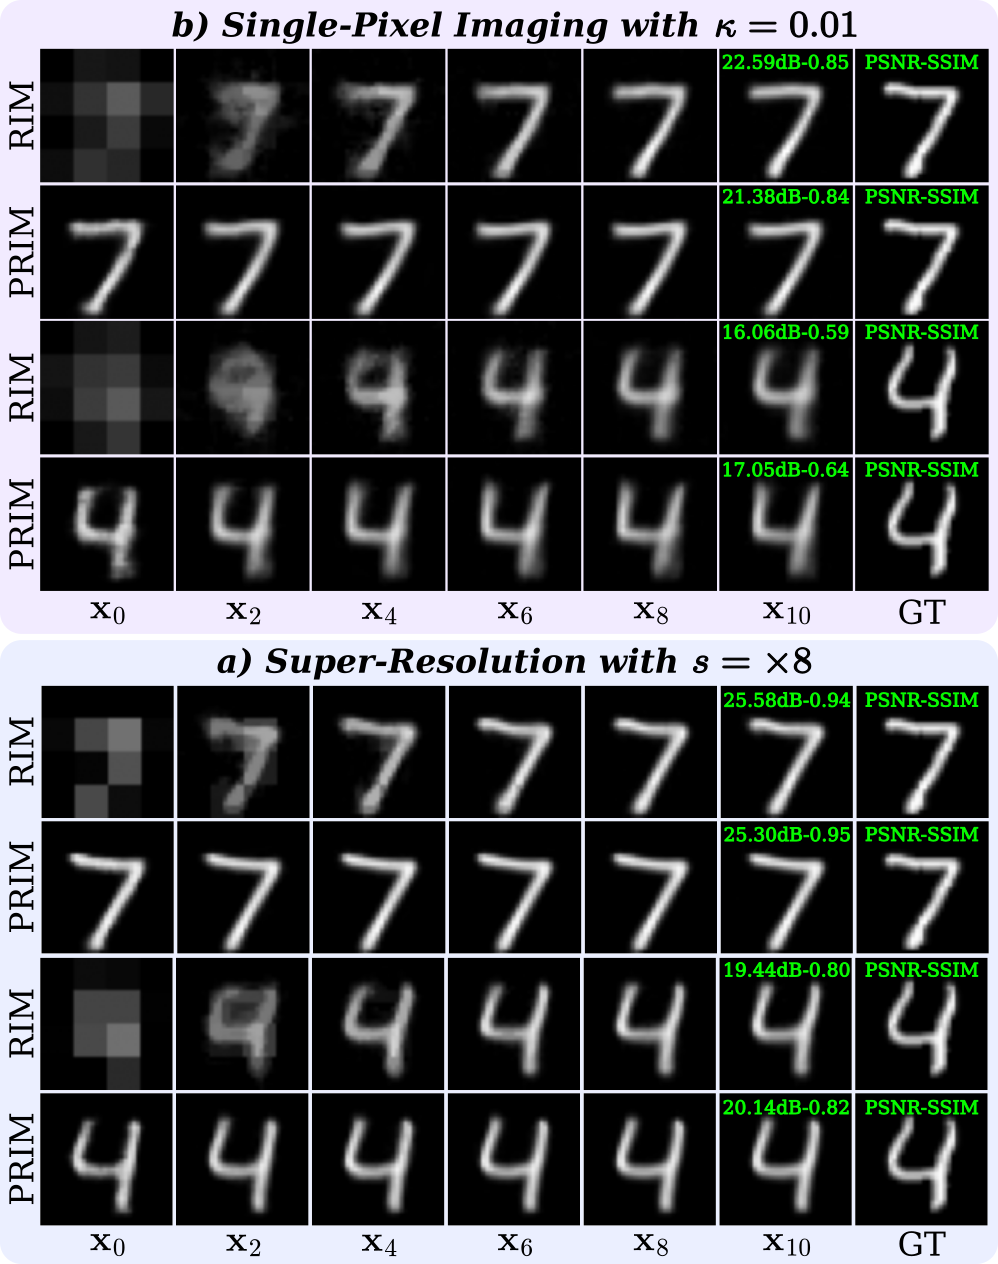
\includegraphics[width=0.49\textwidth]{figures/fig4.png}
    \caption{\textbf{Effect of generative initialization on RIM refinement.} Representative comparison between the standard RIM initialized from the backprojection and PRIM initialized from the fixed encoder-generator pair.}
    \label{fig:rim_prim_comparison}
\end{figure}

For SR, the same trend appears at the more difficult scale factor $s=\times8$. PRIM reaches 20.91 dB PSNR and 0.8590 SSIM, outperforming GANI, PEADMM, and the standard RIM. At $s=\times4$, RIM and PRIM become nearly equivalent in PSNR, with PRIM reaching 29.26 dB and RIM reaching 29.24 dB. In this less ill-posed regime, the standard RIM slightly improves SSIM and MSE, whereas PRIM gives the best MAE. This suggests that the proposed initialization has the largest impact when the observation model removes substantial information, and becomes less decisive as the inverse problem becomes easier. Figure~\ref{fig:qualitative_results} shows representative reconstructions for two challenging scenarios, SPI with $\kappa = 0.01$ and SR with $s=\times 8$, along with enlarged regions and their corresponding PSNR and SSIM values.

In the highly compressed SPI setting, the backprojection $\mathbf{H}^{\top}\mathbf{y}$ exhibits severe structural degradation, consistent with EADMM reaching only 12.58 dB PSNR. ADMM-based methods fail to recover digit structure, while PEADMM provides partial improvements but still exhibits artifacts. GANI produces smoother reconstructions, but tends to deviate locally from the ground truth. In contrast, RIM recovers the overall digit structure more reliably, which is consistent with its higher PSNR of 18.29 dB, although some degree of smoothing is still present. PRIM builds on this behavior and further improves the reconstruction quality. It achieves the best quantitative performance with 18.96 dB PSNR and the highest SSIM, while also producing more continuous strokes and fewer structural artifacts. These visual improvements are in line with the gains reported in Table~\ref{tab:reconstruction_metrics}.

A similar pattern is observed in the SR case with $s=\times 8$. ADMM-based methods fail to reconstruct fine details, whereas GANI generates visually plausible images that are not always well aligned with the ground truth. Both RIM and PRIM provide more accurate reconstructions, with PRIM showing slightly sharper structures and better consistency, consistent with its higher PSNR of 20.91 dB. Overall, PRIM consistently improves over ADMM-based methods and offers modest but reliable gains over the standard RIM, particularly in the most ill-posed scenarios. The visual results follow the same trends as the quantitative metrics, indicating that the proposed initialization leads to more accurate and structurally coherent reconstructions.

\subsection{Effects of Generative Initialization in RIM}

Figure~\ref{fig:rim_prim_comparison} isolates the initialization effect. The standard RIM starts from the backprojection, which preserves measurement information but provides weak image domain structure in highly constrained settings. PRIM instead starts from $\mathcal{G}^{\ast}(\mathcal{E}^{\ast}(\mathbf{H}^{\top}\mathbf{y}))$, giving stronger global digit structure before the same ten recurrent refinement steps. This allows the recurrent updates to focus more on the backprojected measurement residual and local corrections than on recovering coarse digit geometry from the first iterations.

\begin{table}[t!]
\centering
\caption{Single-sample inference runtime. Runtime is reported in ms/img. The Iter. columns indicate ADMM iterations for EADMM/PEADMM, recurrent refinement steps for RIM/PRIM, and one feed-forward pass for GANI.}
\label{tab:inference_runtime}
\setlength{\tabcolsep}{2.2pt}
\renewcommand{\arraystretch}{1.08}
\scriptsize
\resizebox{\columnwidth}{!}{%
\begin{tabular}{|c|cc|cc|cc|cc|}
\hline \hline
\multirow{3}{*}{\textbf{Method}} &
\multicolumn{4}{c|}{\textbf{Single-Pixel Imaging}} &
\multicolumn{4}{c|}{\textbf{Super-Resolution}} \\ \cline{2-9}
&
\multicolumn{2}{c|}{$\kappa=0.01$} &
\multicolumn{2}{c|}{$\kappa=0.05$} &
\multicolumn{2}{c|}{$s=\times 8$} &
\multicolumn{2}{c|}{$s=\times 4$} \\ \cline{2-9}
&
\textbf{Time} & \textbf{Iter.} &
\textbf{Time} & \textbf{Iter.} &
\textbf{Time} & \textbf{Iter.} &
\textbf{Time} & \textbf{Iter.} \\ \hline
\textbf{EADMM} & 18966.8 & 5k & 37878.0 & 10k & 7270.9 & 5k & 14517.8 & 10k \\ \hline
\textbf{PEADMM} & 379.1 & 100 & 68574.3 & 18k & 712.1 & 500 & 6470.7 & 4.5k \\ \hline
\textbf{GANI} & 0.6 & 1 & 0.6 & 1 & 0.5 & 1 & 0.6 & 1 \\ \hline
\textbf{RIM} & 6.2 & 10 & 5.5 & 10 & 5.5 & 10 & 6.2 & 10 \\ \hline
\textbf{PRIM} & 6.0 & 10 & 6.5 & 10 & 6.6 & 10 & 6.7 & 10 \\ \hline \hline
\end{tabular}
}
\vspace{-4mm}
\end{table}

Table~\ref{tab:inference_runtime} reports the single-image runtime. EADMM and PEADMM require thousands of explicit optimization iterations and are therefore orders of magnitude slower than the learned methods in most settings. GANI is the fastest method because it uses only one encoder-generator pass, but its reconstruction quality is consistently below the RIM-based methods. RIM and PRIM both use ten recurrent refinement steps and remain in the millisecond range; importantly, PRIM preserves essentially the same inference cost as the standard RIM while improving reconstruction quality in the most challenging SPI and SR regimes.

\section{Conclusions}

This work proposes PRIM, a RIM-based reconstruction method that uses a fixed learned generative initialization. A pretrained encoder-generator pair maps the backprojected observation to a structured estimate, and an image-space RIM refines it with explicit backprojected measurement residuals. Experiments on SPI and SR show that PRIM improves over ADMM-based baselines and gives the strongest gains in constrained settings, while preserving inference cost close to a standard RIM. The results also show that the benefit of the generator is most relevant when the measurement operator removes substantial information. In easier settings, the standard RIM already recovers most of the structure and PRIM mainly preserves comparable performance. This behavior supports the proposed view of generative initialization as a complementary prior for learned iterative refinement rather than a replacement for data consistency. In addition, the same recurrent architecture is used for RIM and PRIM, so the observed gains can be attributed to the initialization rather than to extra model capacity. Future work will extend this refinement scheme to more complex datasets, richer generators, additional sensing operators, and robustness studies under stronger noise or distribution shifts.

\bibliographystyle{ieeetr}
\bibliography{bibliography}



\end{document}
